
% \section{RESEARCH BACKGROUND AND JUSTIFYING THE TOPIC}
% \subsection{Actuality of Research}
% \subsubsection{Motivation}



 % Цель работы заключается в разработке принципов построения, а также алгоритмического и программного обесп



 
% \subsection{Object Motion}

% \subsubsection{Range sensors}
% \subsubsection*{LiDAR}

% \cite{Mertz2013} provide a good, though somewhat outdated, overview of different approaches to DETECT AND TRACK MOVING OBJECTS (DATMO) using laser scanners. They distinguish between 2D, 2D+ (laser scanners with four scanning planes) and 3D systems.

% % The most obvious way to identify objects is to utilize distance sensors. Different physical principles underlie the many types of sensors. The most often used systems in robotics are LiDAR, ultrasonic, and infrared system. While LiDAR systems continue to be a popular option for DETECT AND TRACK MOVING OBJECTS (DATMO) operations, the first two sensor types are less effective than LiDAR in terms of operating circumstances and resolution.
% % \begin{figure}[H]
% %     \centering
% %     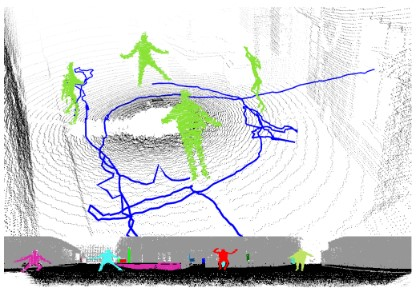
\includegraphics[width=\linewidth/2]{img/Screenshot 2025-01-07 142952.jpg} 
% %     \caption{Lidar data segmentation\citep{Lichtenfeld2024}}
% %     \label{fig:radarsensor}
% % \end{figure}
% % Point grouping, segmentation, data matching, and track updating are the four general processes of LiDAR DATMO techniques \citep{Lichtenfeld2024}. To find a cluster, the data from each survey is first clustered based on predetermined metrics, such as Euclidean distance or intensity. The freshly created clusters are then compared to the tracks of previously tracked items during time.


% \subsubsection{Camera sensors}
% \paragraph{Monocular Camera}
% Vision systems are divided into those using one (monoculars) and more than one video camera. The operation of vision systems using several video cameras is based on the comparison of images of the external environment obtained from two or more spatially separated points of the mobile robot. Due to the spatial separation of the received images in such vision systems, the necessary information about the spatial characteristics of the object is determined. 
% % \begin{figure}[H]
% %     \centering
% %     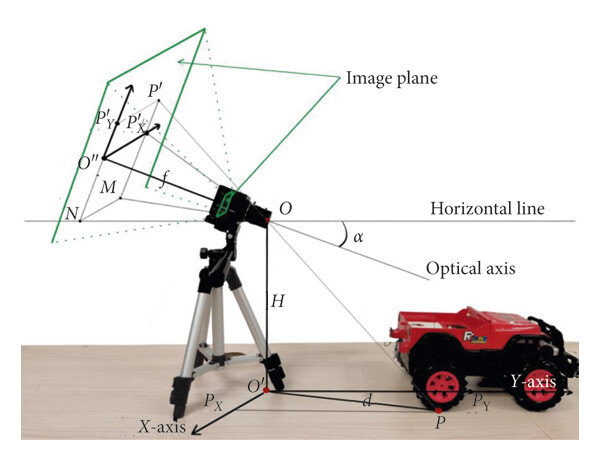
\includegraphics[width=\linewidth/2]{img/scpr9979111-fig-0003-m.jpg} 
% %     \caption{Monocular Vision Ranging\citep{xue2021monocular}}
% %     \label{fig:radarsensor}
% % \end{figure}
% A separate video camera for determining distances to stationary objects can be integrated into the navigation system of a mobile robot. Such a camera focuses on collecting visual data, which is then analyzed to calculate distances to static objects in the robot's environment.

% The use of an additional device can reduce the load on the main image processing system, improve the accuracy of measurements, and improve the reliability of the robot. The specialized camera can be optimized in terms of weight and dimensions, which is especially important in the design of mobile devices where compactness and low weight are critical. At the same time, the robustness and stability of the camera design ensure correct operation in various environments, ensuring stable dimensioning and distance to fixed objects.

% \paragraph{Stereo Camera}
% It is possible to calculate a difference map and extract 3D information from the stereo camera system given two images with a defined baseline. This 3D data makes it possible to specify motion characteristics and measure an object's physical attributes directly.
% % \begin{figure}[H]
% %     \centering
% %     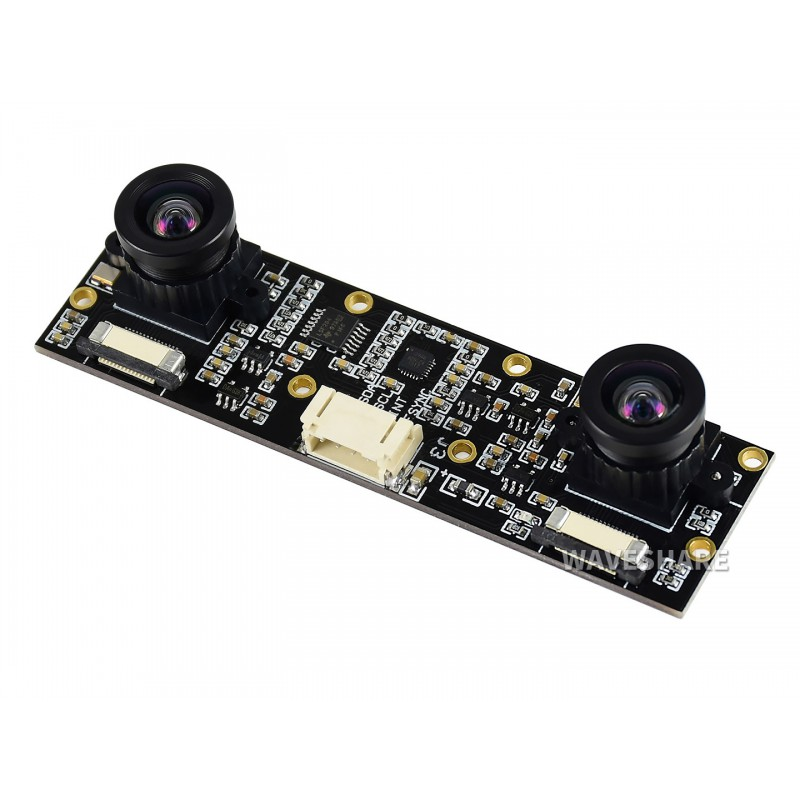
\includegraphics[width=\linewidth/2]{img/imx219-83-stereo-camera-1.jpg} 
% %     \caption{Stereo Camera Module}
% %     \label{fig:radarsensor}
% % \end{figure}

% \subsection{Ego-Motion}
% This is the process of determining the self-motion of a camera or robot in space relative to its environment. Technologies that use sequential image analysis and sensor data to calculate changes in the position and orientation of an object.
% \subsubsection{Inertial systems}
% Similar to the dead reckoning method, inertial navigation systems (INS) obtain pose information by integrating sensor data \citep{biezad1999integrated}. But instead of integrating velocity, ANNs utilize the properties of inertia. Inertial sensors such as INSU (Inertial Measurement Units) give acceleration and angular velocity readings. In order to extract pose data, the acceleration must be indexed twice and the angular velocity must be indexed once \citep{grewal2020global}. 

% % \begin{figure}[H]
% %     \centering
% %     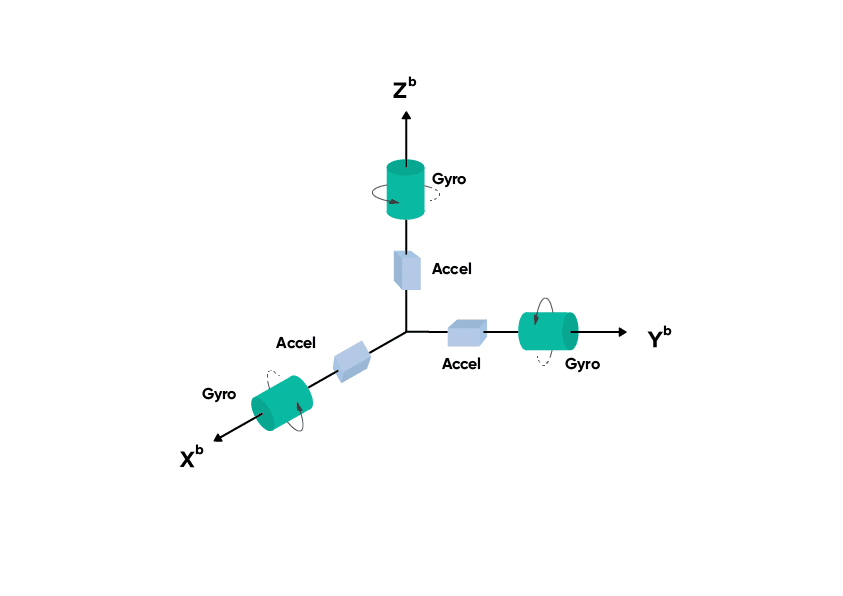
\includegraphics[width=\linewidth]{img/inertial-navigation-systems-ins-an-introduction-img001.png}
% %     \caption{INS}
% %     \label{fig:INS}
% % \end{figure}

% Thus, an ANN is a combination of a sensor and a computing device that performs data filtering and integration. Compared to odometry or dead reckoning, ANN is a relatively new trend in robotics that has emerged due to the recent emergence of accurate and affordable sensors \citep{Borenstein1996WhereAI}.

% \paragraph{Inertial Measurement Unit} are widely used in robotics to measure angular velocities using gyroscopes and accelerations along three axes. Such devices, made by MEMS technology, are cheap, compact, reliable and low-consumption \citep{biezad1999integrated}. IMUs are usually attached rigidly to the robot, so they are called strapdown systems. They detect changes in velocity and orientation relative to the global coordinate system\citep{biezad1999integrated}.

% To track the current pose, the system first integrates angular velocities to determine orientation. The measured accelerations are then converted to the global coordinate system with the influence of gravity removed. This approach allows to accurately determine the position and orientation of the robot in space.


% \subsubsection{Odometry}
% Dead reckoning and odometry are two concepts that are not always easily distinguished. The process of estimating the present pose by integrating velocity and a known heading is sometimes referred to as dead reckoning. Conversely, odometry usually means figuring out the present position using information from "odometer" sensor, the total number of traveled path segments that is acquired from an encoder \citep{Borenstein1996WhereAI}. These phrases are commonly used interchangeably, albeit their definitions can differ. In this thesis, dead reckoning refers to determining the pose by integrating velocity data, whereas odometry particularly refers to calculating the robot's pose by adding up incremental path segments. Both approaches are simple and popular ways to find the position and orientation of a robot \citep{Scaramuzza2011}.

% \paragraph{Encoder Sensors}
% In robotics and control systems, encoders are frequently employed to precisely determine the location and velocity of spinning components. By converting mechanical motion into digital information, encoders make it possible to measure changes in shaft speed, angle, or distance traveled. Measurements are provided by optical or magnetic encoders in modern devices  \citep{Smith2019} .They are capable of measuring absolute or relative. Using the vehicle's geometric characteristics, such as wheel diameter and gear ratio, the recorded angle can be translated into the robot's trip distance \citep{Doe2020}.
% They are extremely challenging to detect quantitatively and to test for \citep{Borenstein1994UMBmarkA}. On the other hand, systematic errors are simpler to handle. They result from inaccurate mechanical components, inadequate comprehension of the system, or approximations in system models. Various calibration methods can be used to estimate and reduce them.

% \paragraph{Optical Speed Sensors}
% Another motion detection technique uses optical sensors and image processing to measure movement speed directly on a 2D surface. This kind of sensor is usually sold as an off-the-shelf device with integrated image processing algorithms, making it simple to access the motion data in its raw form. This technique has the advantage of non-contact measuring, which eliminates the need for mechanical errors and backlashes. This concept of functioning is used by two major kinds of sensors.

% On the one hand, cheap optical motion sensors are frequently found in computer mouse. They are small, use only a few milliwatts of electricity, and have a 10 m/s speed detection range \citep{Logitech2020}. The requirement for a "cooperative" surface, calibration for every individual surface, and a relatively small fixed measured distance are some of the major drawbacks of such sensors.
% % \begin{figure}[H]
% %     \centering
% %     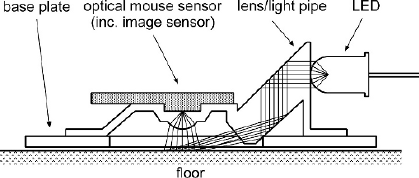
\includegraphics[width=\linewidth/2]{img/Structure-of-optical-mouse-sensor.png}
% %     \caption{Structure of optical mouse sensor}
% %     \label{fig:optical}
% % \end{figure}
% And High-performance solutions, on the other hand, are employed as reference systems in vehicle dynamics research \citep{SensoricSolutions}. Despite their great precision in dry conditions on a level surface, these sensors are relatively big and costly.


% \subsubsection{Visual Odometry}
% Visual odometry is a method of estimating the motion of a robot using sequential images from cameras or lidars \citep{Scaramuzza2011}.

% \paragraph{Waypoint Navigation Systems}
% Navigation systems based on waypoint traversal are currently among the most reliable. However, they have several obvious limitations that significantly restrict their applications. Primarily, these systems are confined to limited spaces, usually indoors, and are prone to errors when unforeseen obstacles appear within the robot's operating area \citep{Borenstein1996WhereAI}. Additionally, maintaining the waypoints (or beacons) requires regular servicing.

% % \begin{figure}[H]
% %     \centering
% %     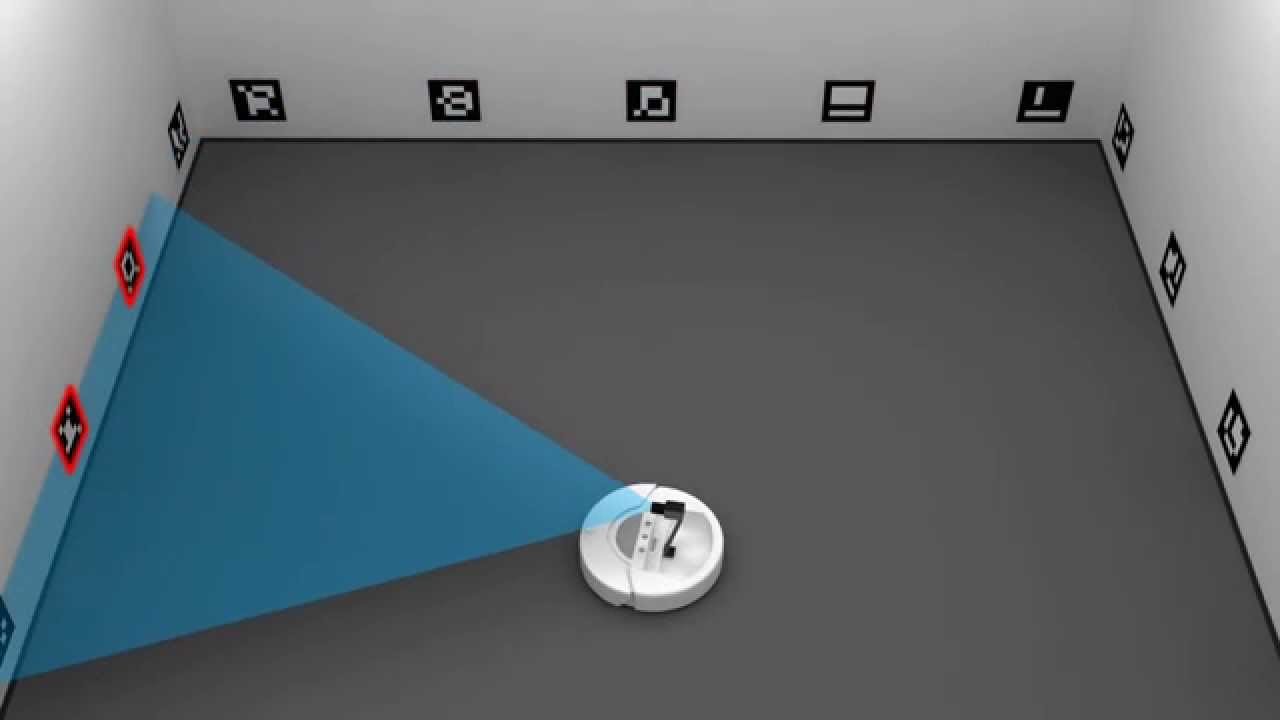
\includegraphics[width=\linewidth/2]{img/maxresdefault.jpg}
% %     \caption{Robot Localization using Waypoint Navigation Systems}
% %     \label{fig:Waypoint}
% % \end{figure}

% \paragraph{Laser and Ultrasonic Range Sensors}
% Another class of rangefinders commonly used in small-scale robots includes laser and ultrasonic range sensors. These are typically employed indoors to perform simple tasks within structured environments . Lidars are limited by the fact that the laser beam only captures data within its line of sight. Small interferences along the beam path can introduce inaccuracies into the generated environmental representation. Ultrasonic sensors, on the other hand, suffer from relatively slow response times, particularly in large open spaces. This limitation prevents robots from moving quickly in such environments.

% \subsubsection{Light Sensor-Based Systems}
% Light sensors range from basic photo-sensitive elements to more sophisticated systems employing video cameras.

% \paragraph{Photo-Sensitive Elements}
% Photo-sensitive elements include components such as photoresistors or infrared (IR) and ultraviolet (UV) receivers. The principle of photoresistors relies on the reduction of resistance with increasing illumination. IR and UV sensors detect obstacles by analyzing light reflected from objects. Using IR and UV LEDs and sensors, obstacles can be detected even before contact because ambient light typically contains minimal radiation at these wavelengths \citep{Logitech2020, SensoricSolutions}.

% \paragraph{Vision-Based Systems}
% Navigation systems that employ video cameras to extract spatial information about the surrounding environment, known as vision-based systems, are particularly noteworthy. Developing such systems is a challenging task, often situated at the intersection of multiple disciplines within artificial intelligence \citep{Jin2019, PointLightYang}. These systems are highly versatile and, in theory, can be equally effective in both indoor and outdoor environments. However, their reliability remains insufficient due to several factors, including susceptibility to various interferences (e.g., vibrations, atmospheric disturbances, optical distortions), the high volume of data to be processed, and the complexity of analyzing the information. These challenges are primarily associated with object recognition issues in the camera's captured images.

% The information processing in such systems generally mimics the human visual apparatus. Spatial data, including obstacle dimensions and distances, is obtained by comparing images captured from two or more viewpoints (stereo vision systems). Based on the disparities between these images, the necessary spatial characteristics of objects are calculated \citep{Smith2019, Doe2020}.

% \paragraph{Rangefinder-Based Systems}
% Active systems are categorized based on the types of sensors they employ: systems using rangefinders (e.g., optical or ultrasonic), light sensors, or solely inertial navigation systems (INS), which operate without analyzing the external environment. An example of an INS is a system using mechanical gyroscopes or accelerometers that measure position, velocity, and acceleration relative to the initial position based on applied forces 
% .

% \paragraph{Contact-Based Systems}
% "Contact-based" systems analyze the environment by detecting obstacles upon collision, triggering a sensor. This allows the robot to map its surroundings and operate within that map. Such systems are typically employed in compact robots \citep{Borenstein1994UMBmarkA}, with a notable example being robotic vacuum cleaners. However, these systems require a pre-created map of the environment, face difficulties accurately determining their own position, and struggle with handling new obstacles that arise after the map has been created.















% The rapid advancement of technology has led to a similarly swift development of drones and an increase in their use for commercial applications. To provide a comprehensive understanding of the current state of this field, this analysis offers an overview of key trends and developments in drone technology. Researchers have analyzed sources to categorize the usage directions of drones. Over the past ten years, general-purpose drones have been the most widespread. However, it's important to note that research in the area of domestic drones shows a negative trend. The authors also highlight the difficulty of analyzing sources in the drone field due to the lack of standardized terminology, with terms like autonomous vehicles, UAV, uncrewed aerial vehicles, UGV, and robot being used interchangeably \cite{hai2020}.

% When considering the use of drones in commerce, particularly in delivery, research indicates a positive trend. Market studies  \cite{dukkanci2020facility} suggest that reducing last-mile delivery costs, which are typically the most expensive for consumers, is a significant driver \cite{boysen2020last}. Current research focuses on reducing costs for UAV-based deliveries. One major challenge is the placement of delivery objects. In the European Union, drone delivery is becoming cheaper, especially in countries like the United Kingdom, Germany, Italy, and France, due to their higher viability thresholds. However, countries like Romania, Hungary, Spain, Latvia, and Bulgaria face regulatory challenges that complicate drone use. Researchers estimate that drone delivery could reduce costs by 15-20\% compared to Amazon's delivery services \cite{aurambout2019last}.

% A third emerging category in the last two to three years is the use of drones for harmful purposes. This issue, discussed by \cite{park2020survey}, highlights the growing threat posed by non-military drones, particularly in civilian areas, due to their potential for illegal and destructive activities. The main proposal involves comprehensive non-military counter-drone systems through existing detection, identification, and neutralization technologies. The goal is to provide recommendations for developing adaptable and effective counter-drone systems that can be deployed in various civilian settings such as airports, sports stadiums, and conference venues. The authors assessed the early stages of non-military counter-drone technology development. Despite technological advances, regulatory and financial constraints limit the widespread adoption of advanced counter-drone systems \cite{park2020survey}.

% In conclusion, while drones have a positive usage trend, their applications are diversifying. Currently, drones are not just toys but tools for various purposes. There is no universal design, as each specific task requires tailored improvements. It's also crucial to consider the potential harm these technologies can cause. Governments are attempting to regulate their widespread use, which can have negative impacts. However, over the years, we can see progress and easing of regulations. Further development is focused on components, sensors, engines, and batteries.



% \begin{itemize}
%     \item Aurambout, JP., Gkoumas, K. & Ciuffo, B., 2019. Last mile delivery by drones: an estimation of viable market potential and access to citizens across European cities. Eur. Transp. Res. Rev., 11, p.30. Available at: https://doi.org/10.1186/s12544-019-0368-2.

% \itemBoysen, N., Fedtke, S. & Schwerdfeger, S., 2020. Last‑mile delivery concepts: a survey from an operational research perspective. Received: 18 May 2020 / Accepted: 4 September 2020 / Published online: 21 September 2020.

% \itemDukkanci, O., Campbell, J.F. & Kara, B.Y., Facility location decisions for drone delivery: A literature review. HAI '20: Proceedings of the 8th International Conference on Human-Agent Interaction, November 2020, pp. 196–203.

% \item Park, S., Kim, H.T., Lee, S., Joo, H. & Kim, H., 2020. Survey on Anti-Drone Systems: Components, Designs, and Challenges. Department of Electrical Engineering, Korea University, Seoul 02841, South Korea. Available at: hnkim@korea.ac.kr. This work was supported by the National Research Foundation of Korea funded by the Korean Government under Grant 2020R1A2C101238.
% \end{itemize}